\begin{figure}[htbp]
    \centering
    \definecolor{waterblue}{RGB}{65,190,225}
    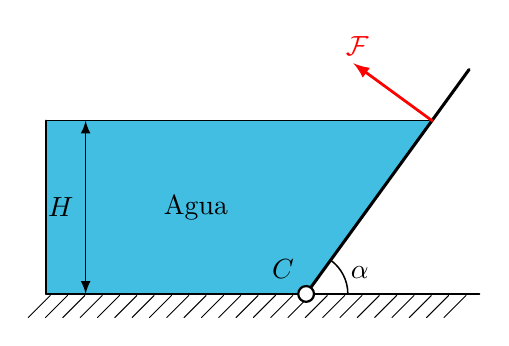
\begin{tikzpicture}[x=1cm,y=1cm,line cap=round,line join=round]
        % Geometría principal
        \coordinate (C) at (3.65,0.45);
        \coordinate (S) at (5.25,2.65);

        % Agua contenida por la compuerta
        \fill[waterblue] (0.35,0.45) -- (C) -- (S) -- (0.35,2.65) -- cycle;
        \draw[line width=0.8pt] (0.35,0.45) -- (0.35,2.65);
        \draw[line width=0.5pt] (0.35,2.65) -- (S);
        \node at (2.25,1.55) {Agua};

        % Suelo y achurado
        \draw[line width=0.8pt] (0.35,0.45) -- (5.85,0.45);
        \foreach \x in {0.40,0.62,...,5.72} {
            \draw[line width=0.35pt] (\x,0.43) -- ++(-0.28,-0.28);
        }

        % Compuerta inclinada y prolongación superior
        \draw[line width=1.1pt] (C) -- (5.72,3.30);

        % Articulación en C
        \fill[white] (C) circle (0.10);
        \draw[line width=0.8pt] (C) circle (0.10);
        \node[above left] at (3.62,0.52) {$C$};

        % Altura del agua
        \draw[latex-latex,line width=0.6pt] (0.85,0.45) -- (0.85,2.65);
        \draw[line width=0.45pt] (0.67,0.45) -- (1.03,0.45);
        \draw[line width=0.45pt] (0.67,2.65) -- (1.03,2.65);
        \node[left] at (0.82,1.55) {$H$};

        % Ángulo alfa entre la compuerta y el suelo
        \draw[line width=0.55pt] (4.18,0.45) arc[start angle=0,end angle=54,radius=0.53];
        \node at (4.33,0.72) {$\alpha$};

        % Fuerza aplicada perpendicularmente a la compuerta
        \draw[red,line width=1.0pt,-latex] (S) -- (4.25,3.38);
        \node[red,above] at (4.30,3.35) {$\mathcal{F}$};
    \end{tikzpicture}
    \caption{Geometría de la compuerta inclinada del problema 5.}
\end{figure}
